\documentclass{tufte-handout}

\title{CIS 2033 Lectures 3 and 4, Spring  2017\thanks{Supplemental reading from Dekking's textbook: \ Chapter 3.}}

\author[David Dobor]{Instructor: David Dobor}

\date{Updated January 24, 2017} % without \date command, current date is supplied

%\geometry{showframe} % display margins for debugging page layout

\usepackage{graphicx} % allow embedded images
  \setkeys{Gin}{width=\linewidth,totalheight=\textheight,keepaspectratio}
  \graphicspath{{graphics/}} % set of paths to search for images
\usepackage{amsmath}  % extended mathematics
\usepackage{amssymb}
\usepackage{booktabs} % book-quality tables
\usepackage{units}    % non-stacked fractions and better unit spacing
\usepackage{multicol} % multiple column layout facilities
\usepackage{lipsum}   % filler text
\usepackage{fancyvrb} % extended verbatim environments
  \fvset{fontsize=\normalsize}% default font size for fancy-verbatim environments

\usepackage{rotating}


% Standardize command font styles and environments
\newcommand{\doccmd}[1]{\texttt{\textbackslash#1}}% command name -- adds backslash automatically
\newcommand{\docopt}[1]{\ensuremath{\langle}\textrm{\textit{#1}}\ensuremath{\rangle}}% optional command argument
\newcommand{\docarg}[1]{\textrm{\textit{#1}}}% (required) command argument
\newcommand{\docenv}[1]{\textsf{#1}}% environment name
\newcommand{\docpkg}[1]{\texttt{#1}}% package name
\newcommand{\doccls}[1]{\texttt{#1}}% document class name
\newcommand{\docclsopt}[1]{\texttt{#1}}% document class option name
\newenvironment{docspec}{\begin{quote}\noindent}{\end{quote}}% command specification environment

\begin{document}

\maketitle% this prints the handout title, author, and date

\begin{abstract}
\noindent
In the first two lectures, we introduced probabilities as a way of describing our beliefs
about the likelihood that a given event will occur. But our beliefs will in general depend 
on the information that we have. Taking into account new information leads us to consider 
the so-called conditional probabilities -- revised probabilities that take into account 
this new information.

Conditional probabilities are very useful whenever we want to break up a model into simpler
pieces using a divide and conquer strategy. This is done using tools that we develop in this lecture
and which we will keep applying throughout this course in different guises. They are also the 
foundation of the field of inference, and we will see how they arise in that context as well.

Next, we will consider a special case where one event does not convey useful information about 
another, a situation that we call \emph{independence}. Independence usually describes
a situation where the occurrence or non-occurrence of different events is determined by factors 
that are completely unrelated. Independence is what allows us to build complex models out of 
simple ones. This is because it is often the case that a complex system is made up of several components
that are affected by unrelated, that is, independent sources of randomness.

And so with the tools to be developed over the next couple of lectures, we will be ready to calculate
probabilities in fairly complex probabilistic models.


\end{abstract}

%\printclassoptions

\section{Introduction}\label{sec:intro}

Suppose I look at the registry of residents of my town and pick a person at random. What is the probability that this person is under 18 years of age? Let's say I find that the answer is about 25\%.

Suppose now that I tell you that this person is married. Will you give the same answer? Of course not. The probability of being less than 18 years old is now much smaller.

What happened here? We started with some initial probabilities that reflect what we know or believe about the world. But we then acquired some additional knowledge, some new evidence-- for example, about this person's family situation.
This new knowledge should cause our beliefs to change, and the original probabilities must be replaced with new probabilities that take into account the new information. These revised probabilities are what we call conditional probabilities. And this is the subject of this lecture.

We will start with a formal definition of conditional probabilities together with the motivation behind this particular definition. We will then proceed to develop three tools that rely on conditional probabilities, including the Bayes rule, which provides a systematic way for incorporating new evidence into a probability model. The three tools that we introduce in this lecture involve very simple and elementary mathematical formulas, yet they encapsulate some very powerful ideas.

It is not an exaggeration to say that much of this class will revolve around the repeated application of variations of these three tools to increasingly complicated situations. In particular, the Bayes rule is the foundation for the field of inference. It is a guide on how to process data and make inferences about unobserved quantities or phenomena. As such, it is a tool that is used all the time, all over science and engineering.

\pagebreak
\section{Conditional Probabilities}\label{sec:CondProbs}

Conditional probabilities are probabilities associated with a revised model that takes into account some
additional information about the outcome of a probabilistic experiment. The question is how to carry out
this revision of our model. We will give a mathematical definition of conditional probabilities, but first let
us motivate this definition by examining a simple concrete example. 



\newthought{Example 1.} Consider a probability model with
12 equally likely possible outcomes -- each outcome has probability equal to 1/12. We will
focus on two particular events, event $A$ and $B$, two subsets of the sample space. Event $A$ has five
elements, so its probability is 5/12, and event $B$ has six elements, so it has probability 6/12.
\begin{marginfigure}
  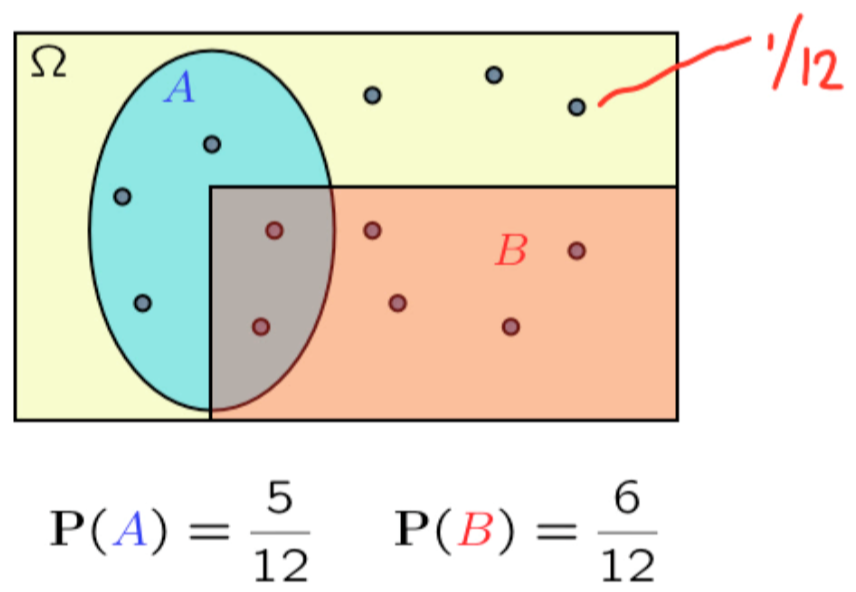
\includegraphics{Cond1}
  \caption{\textbf{Equally Likely Outcomes.} In this model with equally likely outcomes, the probabilities associated with sets $A$ and $B$ are $5/12$ and $1/2$, respectively.}
\end{marginfigure}
\begin{marginfigure}
  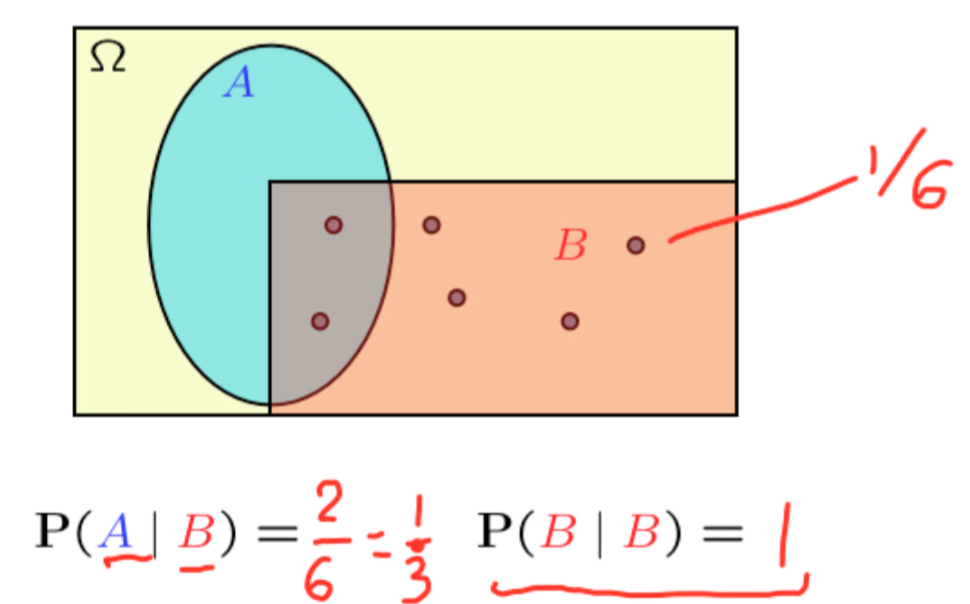
\includegraphics{CondBoccured}
  \caption{\textbf{Event $B$ has occurred.} If is known that $B$ has occurred, we now update our model by assigning 0 probability to the events that are outside of $B$.}
\end{marginfigure}

Suppose now that someone tells you that event $B$ has occurred, but tells you nothing more about the
outcome. \textit{How should the model change?} First, those outcomes that are outside event $B$ are no longer
possible. So we can either eliminate them, as was done in Figure 2, or we might keep them in the
picture but assign them 0 probability, so that they cannot occur.

How about the outcomes inside the event $B$? We're told that one of these 6 outomes inside the event $B$ 
has occurred. Now these 6 outcomes were equally likely in the original model, and there is no reason to change
their relative probabilities. So they should remain equally likely in revised model as well, so each one of
them should have now probability 1/6 since there's 6 of them. And this is our revised model, the
conditional probability law: 

\vspace{3mm}
\textit{$0$ probability to outcomes outside $B$, and probability 1/6 to each one of the
outcomes that is inside the event $B$.}
\vspace{3mm}

Let us write now this down mathematically. We will use the notation $P(A \mid B)$ to describe the conditional
probability of an event $A$ given that some other event $B$ is known to have occurred. We read this
expression as probability of $A$ given $B$. \begin{marginfigure}
  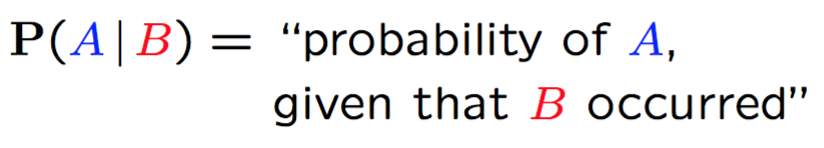
\includegraphics{CondFormula}
\end{marginfigure}So what are these conditional probabilities in our example? In
the new model, where these outcomes are equally likely, we know that event $A$ can occur in two
different ways. Each one of them has probability 1/6. So the probability of event $A$ is 2/6 (i.e. 1/3).



How about event $B$. Well, $B$ consists of 6 possible outcomes each with probability 1/6. So event $B$ in this
revised model should have probability equal to 1. Of course, this is just saying the obvious. Given that
we already know that $B$ has occurred, the probability that $B$ occurs in this new model should be equal to
1. 

\pagebreak
\begin{marginfigure}
  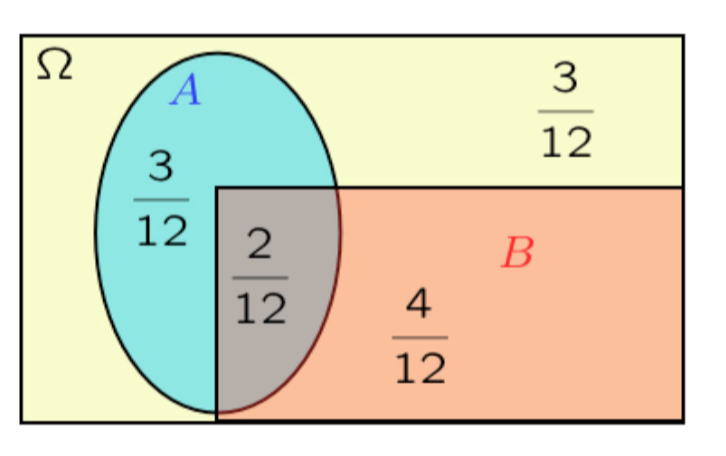
\includegraphics{CondWithProbs}
  \caption{\textbf{Sample Space for Example 2.} The probability distribution here is such that each individual outcome is not necessarily equally likely.}
\end{marginfigure}
\newthought{Example 2.} In this example, the sample space does not consist of equally likely outcomes, but instead we're given
the probabilities of different pieces of the sample space. Notice here that the
probabilities are consistent with what was used in the original example. So this part of $A$ that lies outside
$B$ has probability 3/12, but in this case I'm not telling you how that probability is made up. I'm not telling
you that it consists of 3 equally likely outcomes. So all I'm telling you is that the collective probability in
the blue region in Figure 3 is 3/12.



The total probability of $A$ is, again, 5/12 as before. The total probability of $B$ is 2/12 + 4/12 = 6/12,
exactly as before. So it's a sort of similar situation as before. How should we revise our probabilities and
create -- construct -- conditional probabilities once we are told that event $B$ has occurred?

First, the relation $P(B \mid B) = 1$ should remain true: once we are told that $B$ has occurred, then $B$ is certain to occur,
so it should have conditional probability equal to 1. 

How about the conditional probability  $P(A \mid B)$? Well, we can reason as follows. In the original model, 
and if we just look inside event
$B$, those outcomes that make event $A$ happen had a collective probability which was 1/3 of the total
probability assigned to $B$ (because 2/12 is one-third of 2/12 + 4/12). So out of the overall probability assigned to $B$, 1/3 of that probability
corresponds to outcomes in which event $A$ is happening. Therefore, if I tell you that $B$ has occurred, I
should assign probability equal to 1/3 that event $A$ is also going to happen. So that $P( A \mid B )$ should be equal to 1/3.

\newthought{\textit{Check Your Understanding: }} Are the following statements true of false?
\begin{enumerate}
\item If $\Omega$ is finite and we have a discrete uniform probability law, and if $B \neq \emptyset$, then the conditional probability law on 
$B$, given that $B$ occurred, is also discrete uniform.
\item If $\Omega$ is finite and we have a discrete uniform probability law, and if $B \neq \emptyset$, then the conditional probability law on 
$\Omega$, given that $B$ occurred, is also discrete uniform.
\end{enumerate}

\vspace{3mm}
\begin{turn}{180} 
\color{teal}
\begin{minipage}{\linewidth}
%Answers:
\scriptsize
\begin{enumerate}[(1)]
\item True, because the outcomes inside $B$ maintain the same relative proportions as in the original probability law.
\item False. Outcomes in $\Omega$ that are outside $B$ have zero conditional probability, so it cannot be the case that 
all outcomes in $\Omega$ have the same conditional probability.
\end{enumerate}
\end{minipage}
\end{turn}


\subsection{Definition of Conditional Probability}\label{sec:DefCondProbs}


By now, we should be satisfied that this approach is a reasonable way of constructing conditional
probabilities. But now let us translate our reasoning into a formula. So we wish to come up with a
formula that gives us the conditional probability of an event given another event. 

\begin{marginfigure}
  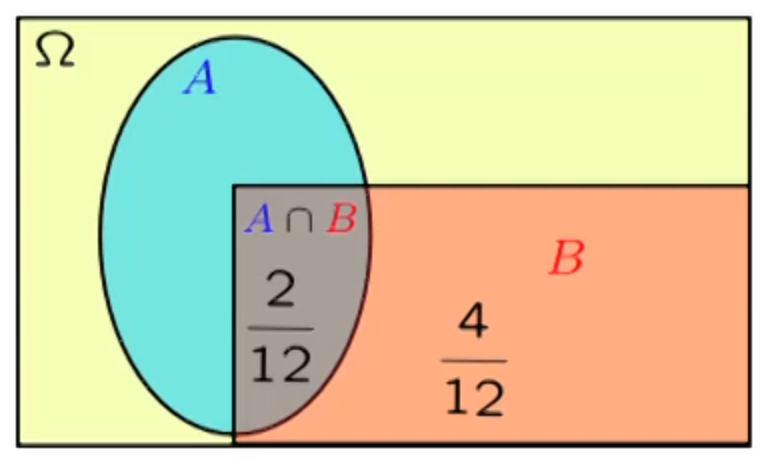
\includegraphics{CondProbDefEg}
\end{marginfigure}

The particular formula
that captures our way of thinking, as motivated before, is the following. Out of the total probability
assigned to $B$, we ask the question, which fraction of that probability is assigned to
outcomes under which event $A$ also happens? So we are living inside event $B$, but within that event, we
look at those outcomes for which event $A$ also happens -- which is the intersection of $A$ and $B$ -- and we
ask: out of the total probability of $B$, what fraction of that probability is allocated to that intersection of $A$
with $B$?



So the following formula captures our intuition of what we did before to construct conditional
probabilities in examples 1 and 2.\begin{figure}
  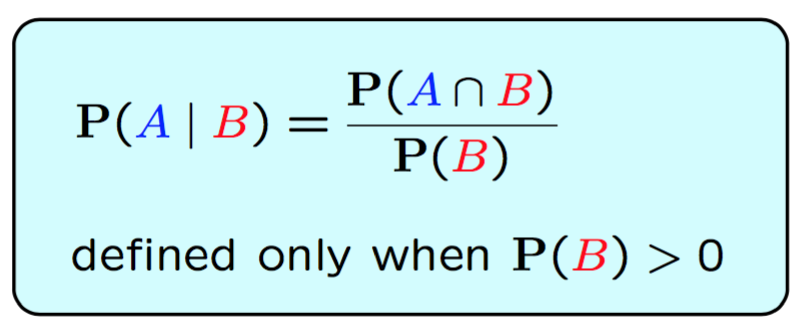
\includegraphics[width=7cm]{CondDef}
  \setfloatalignment{b}
\end{figure}

 Let us check that the definition indeed does what it's supposed
to do. In this example, the probability of the intersection was 2/12 and the total probability of B was
6/12, which gives us 1/3, which is the answer that we had gotten intuitively a little earlier.


As a side point, let me also make a comment that this definition of conditional probabilities makes sense
only if we do not attempt to divide by zero, i.e. only if the event B on which we're conditioning has
positive probability. If event B has 0 probability, then conditional probabilities given B will be left
undefined.

And one final comment. This is a definition. It's not a theorem. What does that mean? It means that
there is no question whether this equality is correct or not. It's just a definition. There's no issue of
correctness. The earlier argument that we gave was just a motivation of the definition. We tried to figure
out what the definition should be if we want to have a certain intuitive and meaningful interpretation of
the conditional probabilities. Let us now continue with a simple example.


\vspace{0.5cm}


\newthought{Example 3.} This is a example where we want to just apply the formula for conditional probabilities and see
what we get. The example involves a four-sided die, which we roll
twice, and we record the first roll, and the second roll. So there are 16 possible outcomes. 
We assume, to keep things simple, that each one of those 16 possible outcomes has
the same probability, so each outcome has the probability 1/16. 

\begin{marginfigure}
  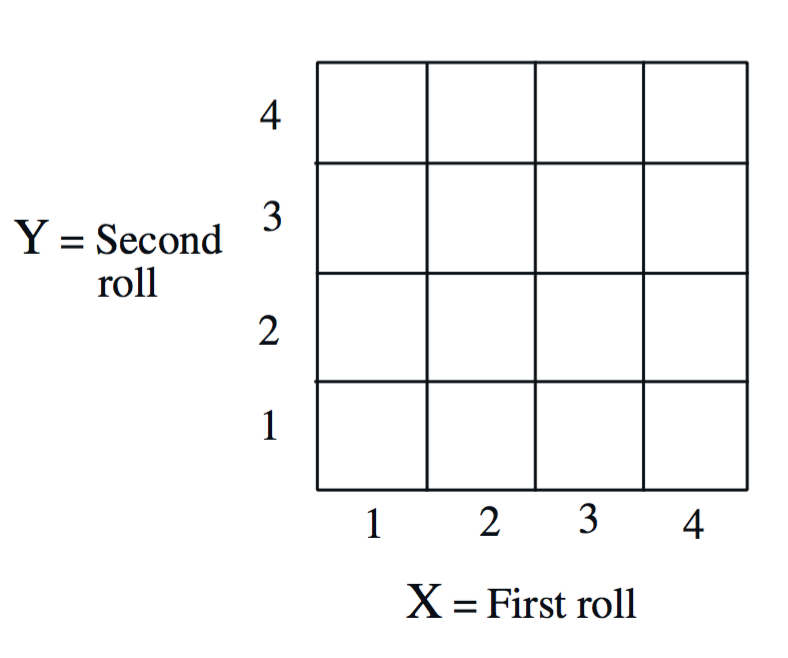
\includegraphics{TetraDie}
  \caption{\textbf{Tetrahedral die, again.}}
  \setfloatalignment{b}
\end{marginfigure}
Let us consider now a particular event
$B$ on which we're going to condition. This is the event under which the smaller of the two die rolls is
equal to 2, which means that one of the dice must have resulted in two, and the other die has resulted
in something which is 2 or larger.

\begin{figure}
  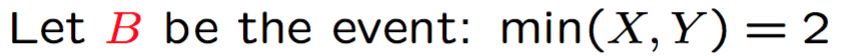
\includegraphics[width=8cm]{MinFormula}
  \setfloatalignment{b}
\end{figure}

Event $B$ can happen in multiple ways: at 2, 2, or
2, 3, or 2, 4; then a 3, 2 and a 4, 2. All of these are outcomes in which one of the dice has a value equal
to 2, and the other die is at least as large.


So we condition on event $B$. This results in a conditional model where each one of those five
outcomes (pink squares in Figure 5) are equally likely since they used to be equally likely in the original model. 

Now let's look at another quantity, let's call it $M$, the maximum of the two die rolls -- that is, the largest of the results. 

\begin{figure}
  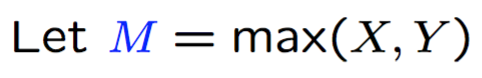
\includegraphics[width=5cm]{MaxFormula}
  \setfloatalignment{b}
\end{figure}


We now would like to calculate the conditional probability that the maximum is equal to 1 given that the minimum is
equal to 2:

$$ P (M = 1 \mid B = 2) $$



Well, such outcome cannot happen! If I tell you that the smaller number is 2, then the larger
number cannot be equal to 1, so this outcome is impossible, and therefore this conditional probability is
equal to $0$. 

$$ P (M = 1 \mid B = 2) = 0$$

Let's do something a little more interesting.

\begin{marginfigure}
  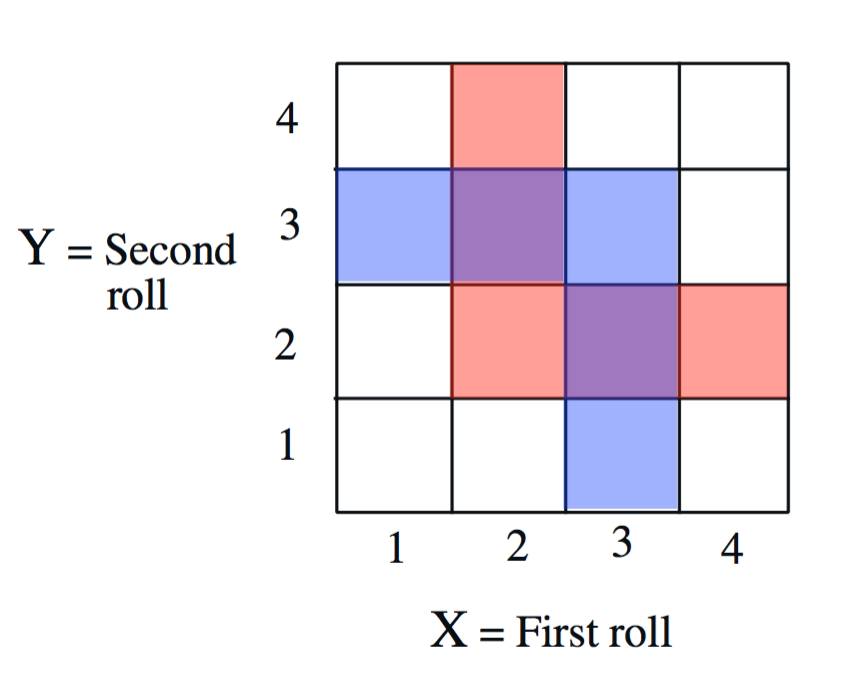
\includegraphics{ColoredDie1}
  \caption{\textbf{Tetrahedral die.} Pink squares correspond to event $B$. Blue squares -- to event $A$.}
  \setfloatalignment{b}
\end{marginfigure}

Let us now look at the conditional probability that the maximum is equal to 3, given the information that
event $B$ has occurred. It's best to draw a picture and see what that event corresponds to. $M$ is equal to
3 -- the maximum is equal to 3 -- if one of the dice resulted in a 3, and the other die resulted in
something that's 3 or less. So this event here corresponds to the blue region in this diagram.

Now let us try to calculate the conditional probability by just following the definition. The conditional
probability of one event given another is the probability that both of the two events 
occur, divided by the probability of the conditioning event. That is, out of the total probability in the
conditioning event, we ask, what fraction of that probability is assigned to outcomes in which the event
of interest is also happening?

So what is this event? The maximum is equal to 3, which is the blue event. And simultaneously, the pink
event is happening. These two events intersect only in two places. Figure 5 shows the intersection of the two
events - these are the squares that are shaded both blue and pink. And the probability of that intersection is 
2 out of 16, since there are 16 outcomes and that event
happens only with two particular outcomes. So this gives us 2/16 in the numerator.

How about the denominator? Event $B$ consists of a total of five possible outcomes. Each one has
probability 1/16, so this is 5/16. Thus the final answer is 2/16 divided by 5/16, or 2/5.

We could have gotten that same answer in a simple and perhaps more intuitive way. In the original
model, all outcomes were equally likely. Therefore, in the conditional model, the five outcomes that
belong to $B$ should also be equally likely. Out of those five, there are two of them that make the event of
interest to occur. So given that we live in $B$, there's two ways out of five that the event of interest will
materialize. So the event of interest has conditional probability equal to 2/5.


\newthought{\textit{Check Your Understanding: }} Let the sample space be the unit square, $\Omega  = [0, 1]^2$, and
and let the probability of a set be the area of the set. Let $A$ be the set of points $(x, y) \in [0, 1]^2$ for which $y \leq x$.
Let $B$ be the set of points for which $x \leq 1/2$. Find $P(A \mid B)$.

\begin{turn}{180} 
\color{teal}
\begin{minipage}{\linewidth}
%Answer:
\scriptsize
theanswerisonefourth%$P(A \mid B) = 1/4$
\end{minipage}
\end{turn}


\vspace{0.4cm}
\subsection{Conditional Probabilities Obey the Same Axioms}\label{sec:CondAxioms}

\textit{(Skim this section on first reading.)}

\vspace{0.4cm}

\noindent We want to emphasize an important point. Conditional probabilities are just the same as ordinary
probabilities applied to a different situation. They do not taste or smell or behave any differently than
ordinary probabilities. What do I mean by that?


\vspace{0.2cm}


\begin{marginfigure}
  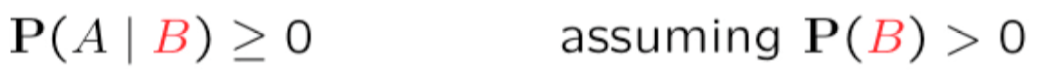
\includegraphics{CondProbAx1}
  \caption{Conditional probabilities also satisfy the familiar axioms. This one was axiom 1.}
  \setfloatalignment{b}
\end{marginfigure}

\textit{Axiom 1.} I mean that they satisfy the usual probability axioms. For example, ordinary probabilities must be
non-negative. Is this true for conditional probabilities? Of course it is true, because conditional
probabilities are defined as a ratio of two probabilities. Probabilities are non-negative. So the ratio will
also be non-negative, of course as long as it is well-defined. And here we need to remember that we
only talk about conditional probabilities when we condition on an event that itself has positive
probability.

\vspace{0.2cm}

\textit{Axiom 2.} Let's check it out the second axiom - what is the probability of the entire sample space, given the event $B$?  
By definition, the conditional probability is the probability of the intersection of the two
events involved divided by the probability of the conditioning event. Now, what is the intersection of
$\Omega$ with $B$? $B$ is a subset of $\Omega$. So when we intersect the two sets, we're left just with $B$ itself.


So the numerator becomes the probability of $B$. We're dividing by the probability of $B$, and so the
answer is equal to 1. So indeed, the sample space has unit probability, even under the conditional
model.

Now, remember that when we condition on an event $B$, we could still work with the original sample
space. However, outcomes that do not belong to $B$ are considered impossible, so we might as
well think of $B$ itself as being our sample space.

\begin{marginfigure}
  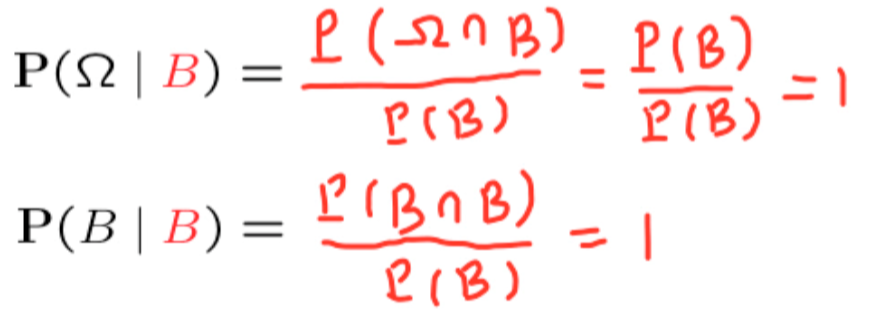
\includegraphics{CondProbAx2}
  \caption{And this one was axiom 2.}
  \setfloatalignment{b}
\end{marginfigure}

If we proceed like that and think now of $B$ as being our new sample space, what is the probability of this
new sample space in the conditional model? Let's apply the definition once more. It's the probability of
the intersection of the two events involved, $B$ intersection $B$, divided by the probability of the
conditioning event.

What is the numerator? The intersection of $B$ with itself is just $B$, so the numerator is the probability of $B$.
We're dividing by the probability of $B$. So the answer is, again, 1. 

\vspace{0.2cm}

\textit{Axiom 3.} Finally, we need to check the additivity axiom. Recall what the additivity axiom says. If we have two
events, two subsets of the sample space that are disjoint, then the probability of their union is equal to
the sum of their individual probabilities. Is this going to be the case if we now condition on a certain
event? 

What we want to prove is the following statement. If we take two events that are disjoint (they have empty intersection)
then the probability of the union is
the sum of their individual probabilities, but where now the probabilities that we're employing are the
conditional probabilities, given the event $B$. That is, we want to show that
$$
\text{If } A \cap C  = \varnothing \text{ then } P( A \cup C \mid B) = P (A \mid B) + P (C \mid B)
$$


So let us verify whether this relation is correct or not.

By definition,
\begin{equation}
 P( A \cup C \mid B) = \frac{P \left( (A \cup C ) \cap B \right)}{P(B)}
\end{equation}

Now, let's look at this quantity, what is it?

We take the union $A \cup C$, and then intersect it with $B$. The result consists 
of the two gray pieces in Figure 8 .

\begin{marginfigure}
  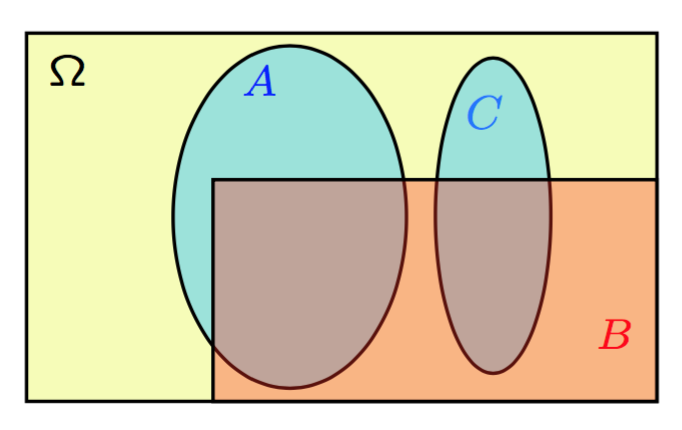
\includegraphics{CondProbAx3}
  \caption{And this picture illustrates axiom 3 for conditional probabilities.}
  \setfloatalignment{b}
\end{marginfigure}

So we rewrite expression (1) as follows:
\begin{align*}
 P( A \cup C \mid B) &= \frac{P \left( (A \cup C ) \cap B \right)}{P(B)} \\
 &= \frac{P \left( (A \cap B) \cup (C \cap B) \right)}{P(B)}
\end{align*}

OK, now here's an observation. We assumed that the events $A$ and $C$ were disjoint. Then the piece
of $A$ that also belongs in $B$, therefore, is disjoint from the piece of C that also belongs to $B$.

Since $A \cap B$ and $C \cap B$ are disjoint, the probability of their
union has to be equal to the sum of their individual probabilities. So here we're using the additivity
axiom on the original probabilities to break this probability up into two pieces. 

Thus we continue the previous expression as follows:
\begin{align*}
\frac{P \left( (A \cap B) \cup (C \cap B) \right)}{P(B)} &= \frac{P (A \cap B)  + P (C \cap B)}{P(B)}\\
 &= \frac{P (A \cap B)}{P(B)}  + \frac{P (C \cap B)}{P(B)}
\end{align*}

And now we observe that here we have ratios of probabilities of intersections by the probability of $B$. 
So we see that the first term is just
the conditional probability $P( A \mid B)$, using the definition of conditional probabilities. Similarly, the second
part is just $P( C \mid B)$. 

\vspace{0.2cm}
So we have indeed checked that this additivity property is true for the case of conditional
probabilities when we consider two disjoint events. 
\vspace{0.2cm}

Now, we could repeat the same derivation and verify that it is also true for the case of a disjoint union
of finitely many events, or even for countably many disjoint events. We're not proving it, but the argument 
is exactly the same as for the case of two events.

\vspace{0.2cm}
\textit{To conclude,} conditional probabilities do satisfy all of the standard axioms of probability theory. So conditional
probabilities are just like ordinary probabilities.

\vspace{0.2cm}
This actually has a very important implication. Since conditional probabilities satisfy all of the probability
axioms, any formula or theorem that we ever derive for ordinary probabilities will remain true for
conditional probabilities as well.

\pagebreak

\section{Models Based on Conditional Probabilities}\label{sec:models}

Let us now examine what conditional probabilities are good for. We have already discussed that they
are used to revise a model when we get new information, but there is another way in which they arise.
We can use conditional probabilities to build a multi-stage model of a probabilistic experiment. We will
illustrate this through an example involving the detection of an object up in the sky by a radar. We will
keep our example very simple. On the other hand, it turns out to have all the basic elements of a real-world
model.



So, we are looking up in the sky, and either there's an airplane flying up there or not. Let us call Event $A$
the event that an airplane is indeed flying up there:

$$
\text{Event } A: \ \text{Airplane is flying above,}
$$
and we have two possibilities: either event $A$ occurs,
or the complement of $A$ occurs, in which case nothing is flying up there. At this point, we can also assign
some probabilities to these two possibilities. Let us say that through prior experience, perhaps, or some
other knowledge, we know that the probability that something is indeed flying up there is 5\% and with
probability 95\% nothing is flying.


\begin{marginfigure}
  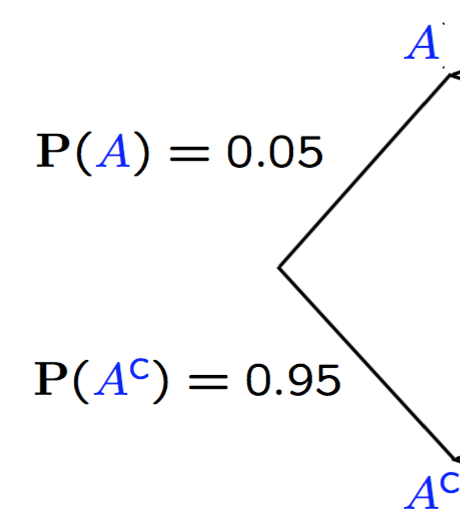
\includegraphics{AirplaneTree1}
  \setfloatalignment{b}
\end{marginfigure}


\vspace{0.2cm}
Now, we also have a radar that looks up into the sky. Let event $B$ be that the radar detects something:
$$
\text{Event } B: \ \text{Something registers on the radar screen}
$$

There are two things that can happen:  either
something registers on the radar screen or nothing registers. Of course, if it's a good radar, probably
event $B$ will tend to go together with event $A$. But it's also possible that the radar will make some
mistakes.


And so we have various possibilities. If there's a plane up there, it's possible that the radar will detect it,
in which case event $B$ will also happen. But it's also conceivable that the radar will not detect it, in which
case we have a so-called miss. So "miss" happens if a plane is flying up there, but the radar does not detect
it. 

\begin{marginfigure}
  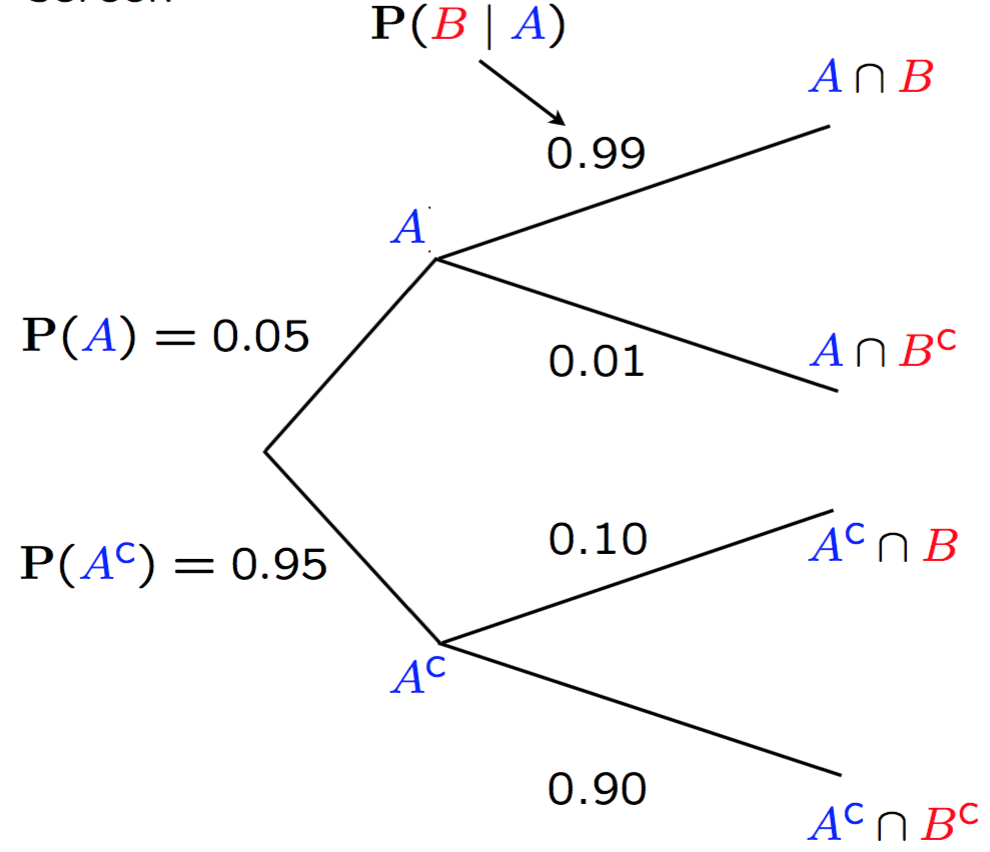
\includegraphics{AirplaneFullTree}
  \caption{Event $A \cap B^c$ is called a "\textit{miss}". Event $A^c \cap B$ is called a "\textit{false alarm}". Pause here a second and make sure this terminology makes sense to you.}
  \setfloatalignment{b}
\end{marginfigure}



Another possibility is that nothing is flying up there, but the radar does detect something, and this is a
situation that's called a \textit{false alarm}. Finally, there's the possibility that nothing is flying up there, and the
radar did not see anything either.

\pagebreak
\begin{marginfigure}
  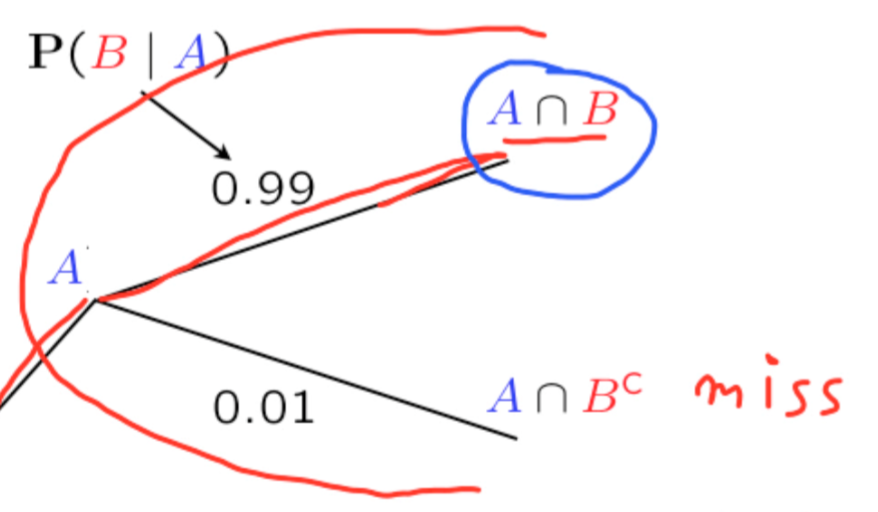
\includegraphics{AirplaneTreePart1}
  \caption{Part of the tree where Event $A$ has occurred. This is the upper part of Figure 9 on the previous page.}
  \setfloatalignment{b}
\end{marginfigure}


Now, let us focus on one particular situation. Suppose that event $A$ has occurred. 
In this universe where event $A$ has occurred, there are two possibilities, and we can assign probabilities to
these two possibilities. Let's say that if something is flying up there, our radar will find it with
probability 99\%, but will also miss it with probability 1\%. 

What's the meaning of this number, 99\%? Well, this is a probability that applies to a situation where an
airplane is up there. So it is really a conditional probability: It's the conditional probability that the radar 
will detect the plane, given that the plane is already flying up there. And
similarly, this 1\% can be thought of as the conditional probability that the complement of $B$ occurs, so
the radar doesn't see anything, given that there is a plane up in the sky.


We can assign similar probabilities under the other scenario. If there is no plane, there is a probability
that there will be a false alarm, and there is a probability that the radar will not see anything. 

These four
numbers  -- $P(B \mid A), P(B^c \mid A),  P(B \mid A^c), P(B^c \mid A^c)$ -- are, in essence, the specs of our radar. 
They describe how the radar behaves in a world
in which an airplane has been placed in the sky, and some other numbers that describe how the radar
behaves in a world where nothing is flying up in the sky.

\begin{marginfigure}
  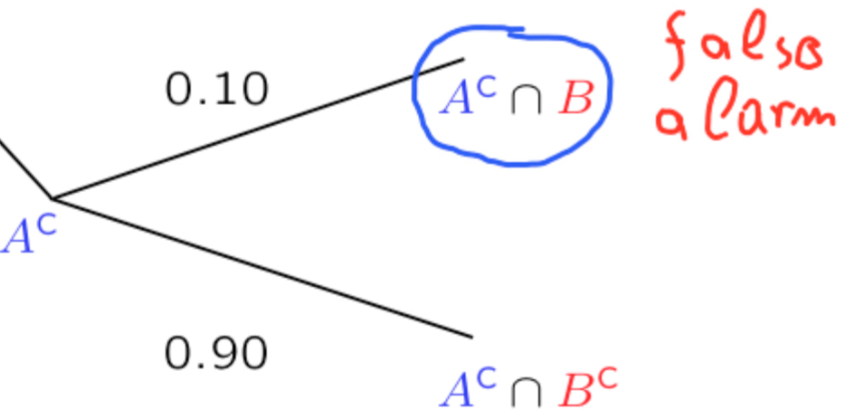
\includegraphics{AirplaneTreePart2}
  \caption{Part of the tree where event $A^c$ has occurred. This is the lower part of Figure 9 on the previous page.}
  \setfloatalignment{b}
\end{marginfigure}


\vspace{0.3cm}
So we have described various probabilistic properties of our model, but is it a complete model? Can we
calculate anything that we might wish to calculate? 

For example, can we calculate the
probability that both $A$ and $B$ occur? This corresponds to reaching the upper right leaf of the tree in
Figure 9 or Figure 10, the one labeled $A \cap B$. How can we calculate it?

Well, let us remember the definition of conditional probabilities. The conditional probability of an event
given another event is the probability of their intersection divided by the probability of the conditioning
event: 
$$
P(B \mid A) = \frac{P(B \cap A)}{P(A)}
$$
Or, rearranging, 
$$
P(A \cap B) = P(B \cap A) = P(B \mid A) P(A)
$$

So, in words, the probability that $A$ and $B$ occur is equal to the probability that $A$ occurs times the
conditional probability that $B$ occurs given that $A$ occurred.  And in our example, this is 
$$
P(B \mid A) P(A) = 0.99 \times 0.05 
$$

Before we go on, let me take a moment to rewrite this for nicer looks. (Heads up: It helps on quizzes to know these 
nside out.) We have:

\begin{figure}
  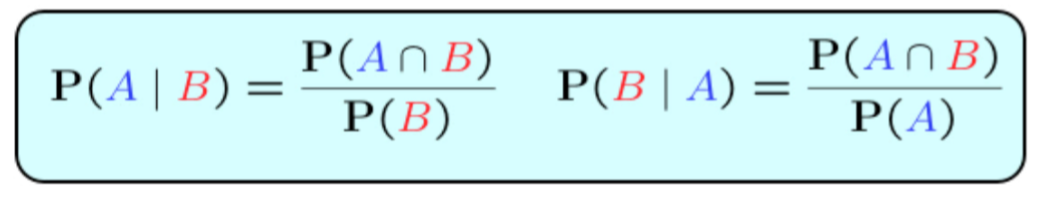
\includegraphics{DefCondProbs}
\end{figure}


So we can calculate the probability of event $A \cap B$ by multiplying probabilities and conditional
probabilities along the path in the tree diagram that leads us to the top right leaf. 

\begin{marginfigure}
  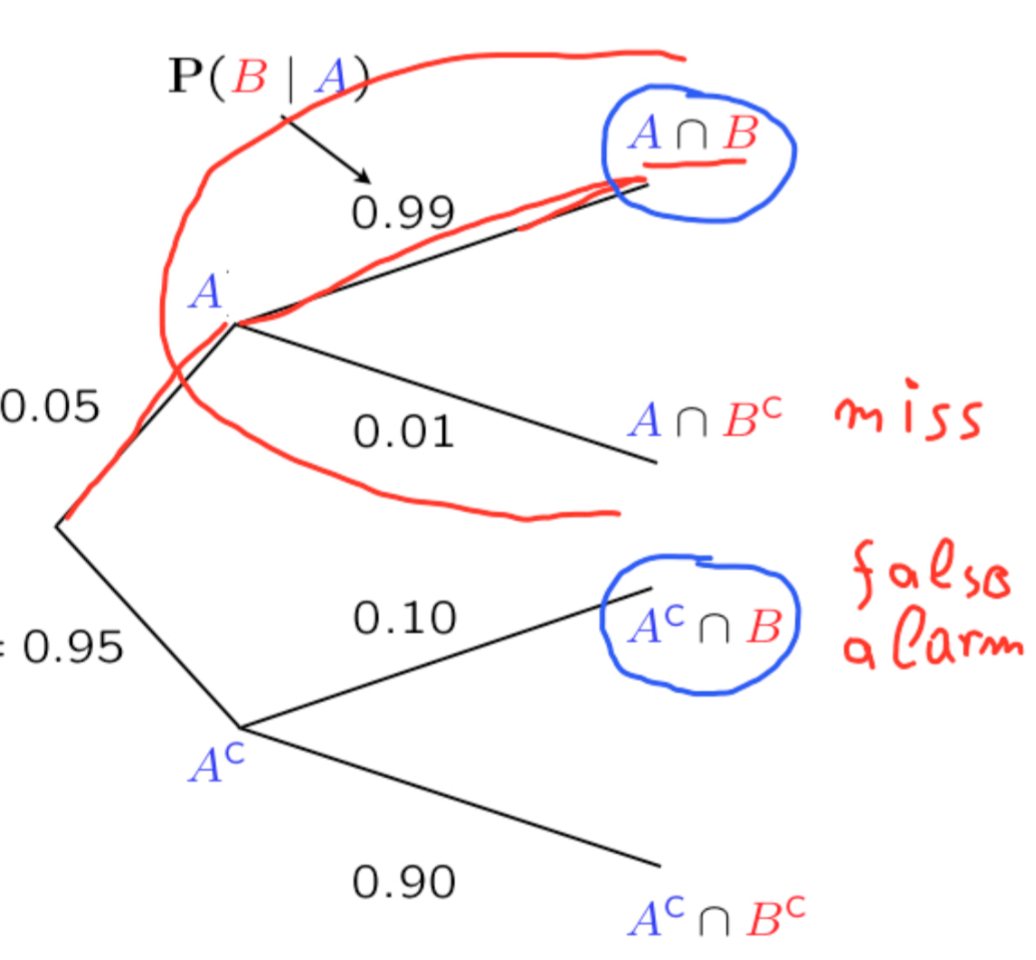
\includegraphics{TreeBranchesRed}
  \caption{The branches leading to event $A \cap B$ are traced in red.}
  \setfloatalignment{b}
\end{marginfigure}

And we can do the same for any
other leaf in this diagram. So for example, the probability that $A^c \cap B^c$ happens is going to be the probability
event $A^c$ times the conditional probability $P (B^c \mid A^c)$. 

So you could trace these two branches too to get the probability 0.95 $\times$ 0.90 = 0.855 of event $A^c \cap B^c$ occurring. 

\vspace{0.2cm}
How about a different question? What is the probability, the total probability, that the radar sees
something? Let us try to identify this event. The radar can see something under two scenarios:
\begin{enumerate}
\item A plane is up in the sky and the radar sees it.
\item Nothing is up in the sky, but the radar thinks that it sees something. 
\end{enumerate}

These two possibilities together make up the event $B$.

\vspace{0.2cm}
And so to calculate the probability of $B$, we need to add the probabilities of these two events. 

For the first event, we already calculated its probability. It's 0.05 $\times$ 0.99. For the second possibility, we need to do a
similar calculation. The probability that this second event occurs is equal to 0.95 times the conditional probability of $B$
occurring under the scenario where $A^c$ has occurred, and this is 0.10. So we have $P(A^c \cap B) = $ 0.95 $\times$ 0.10. 

We add those two
numbers together, the answer turns out to be:

\begin{align*}
P (B) &= P(A) P(B \mid A) + P(A^c) P(B \mid A^c) \\
         & =  0.05 \times 0.99 + 0.95 \times 0.10\\
         &= 0.1445
\end{align*}


\vspace{0.2cm}
\textit{Finally}, the last question, which is perhaps the most interesting one. Suppose that the radar registered
something. What is the probability that there is an airplane up there? How do we do this calculation?
Well, we can start from the definition of the conditional probability of $A$ given $B$, and note that we already
have in our hands both the numerator and the denominator.

\begin{align*}
P(A \mid B) &= \frac{P(A \cap B)} {P(B) }\\
                   & = \frac{0.05 \times 0.99} {0.05 \times 0.99 + 0.95 \times 0.10}\\
                   & = \frac{0.0495}{0.1445}\\
                   & = 0.3426
\end{align*}

\vspace{0.2cm}
So there is a 34\% probability that an airplane
is there given that the radar has seen or thinks that it sees something.

\vspace{0.2cm}
\textit{Now, the numerical value of this answer is somewhat interesting}  because it's pretty small. Even though we
have a very good radar that tells us the right thing 99\% of the time under one scenario and 90\% under
the other scenario. Despite that, given that the radar has seen something, this is not really convincing
or compelling evidence that there is an airplane up there. The probability that there's an airplane up
there is only 34\% in a situation where the radar thinks that it has seen something.

\vspace{0.2cm}
In the next few segments, we are going to revisit these three calculations and see how they can
generalize. In fact, a large part of what is to happen in the remainder of this class will be elaboration on
these three ideas. They are three types of calculations that will show up over and over, of course, in
more complicated forms, but the basic ideas are essentially captured in this simple example. 

\pagebreak
\section{Multiplication Rule}\label{sec:MultRule}

As promised, we will now start developing generalizations of the different calculations that we carried
out in the context of the radar example. The first kind of calculation that we carried out goes under the
name of the multiplication rule. And it goes as follows. Our starting point is the definition of conditional
probabilities.

The conditional probability of $A$ given another event, $B$, is the probability that both events have occurred
divided by the probability of the conditioning event. 

\begin{align*}
P(A \mid B) &= \frac{P(A \cap B)} {P(B) }\\
\end{align*}

We now take the denominator term and send it to
the other side of this equality to obtain this relation
\begin{align*}
P(A \cap B) = P(A \mid B) P(B)\\
\end{align*}

\noindent which we can interpret as follows. The probability
that two events occur is equal to the probability that a first event occurs, event $B$ in this case, times the
conditional probability that the second event, event $A$, occurs, given that event $B$ has occurred.

Now, out of the two events, $A$ and $B$, we're of course free to choose which one we call the first event
and which one we call the second event. So the probability of the two events happening is also equal to
an expression of this form

\begin{align*}
P(A \cap B) = P(B \mid A) P(A) \\
\end{align*}



\begin{marginfigure}
  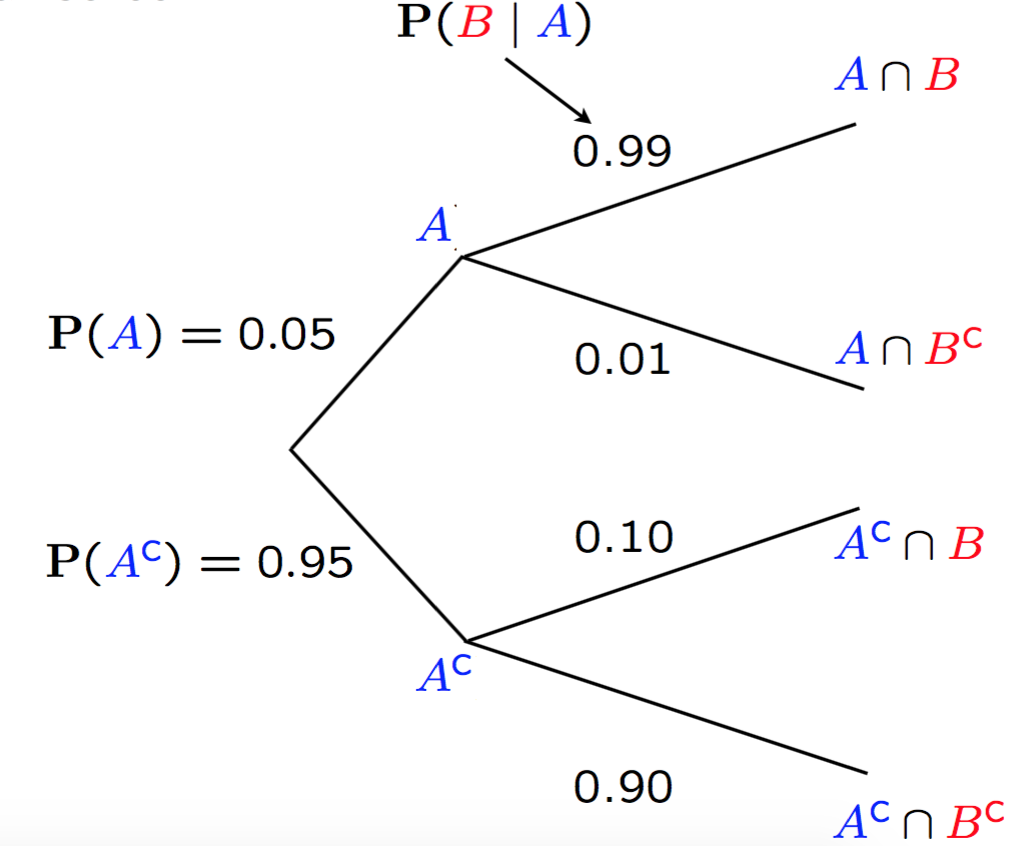
\includegraphics{TreeAgain}
  \caption{Same tree diagram as before.}
  \setfloatalignment{b}
\end{marginfigure}


We used this formula in the context of a tree diagram, and we used it to calculate the probability of the
$A \cap B$ leaf of 
this tree by multiplying the probability of taking the
branch labeled $P(A)$ and multiplying that probability by the the conditional probability of taking the branch
goint from $A$ to $A\cap B$, which is the
probability that event B also occurs given that event A has occurred, i.e. $P(B \mid A)$.

\vspace{0.2cm}
\textit{How do we generalize this calculation?} Consider a situation in which the experiment has an additional
third stage that has to do with another event, C, that may or may not occur.

\pagebreak
\begin{marginfigure}
  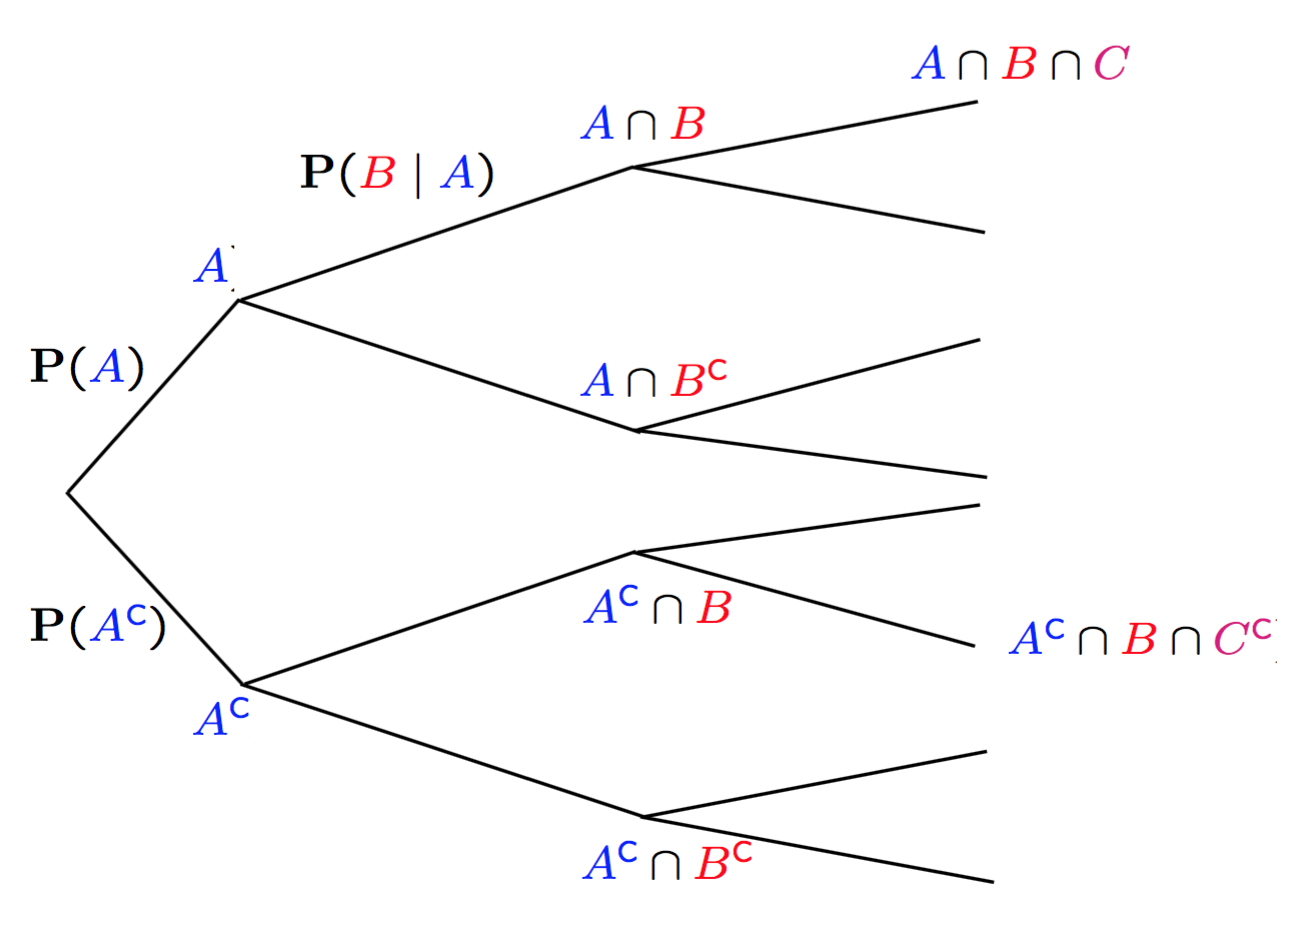
\includegraphics{GeneralizedTree}
  \caption{Here our experiment has the third stage that has to do with another event $C$.}
  \setfloatalignment{b}
\end{marginfigure}


For example, if we have arrived at the node labeled $A \cap B$, $A$ and $B$ have both occurred. Next, if $C$ also occurs, then we
reach the leaf of the tree that is labeled $A \cap B \cap C$. Or there could be other scenarios. For example, it could be the
case that $A$ did not occur. Then event $B$ occurred, and finally, event $C$ did not occur, in which case we
end up at the leaf labeled $A^c \cap B \cap C^c$.

What is the probability of this scenario happening? Let us try to do a calculation similar to the one that
we used for the case of two events. However, we need to deal here with three events. What should we
do? Well, we look at the intersection of these three events and think of it as the intersection of a
composite event, $A^c \cap B$, then intersected with the event $C^c$. 

$$
P(A^c \cap B \cap C^c) = P\left( (A^c \cap B) \cap C^c \right)
$$


Clearly, you can form the intersection of three events by first taking the intersection of two of them and
then intersecting with a third. After we group things this way, we're dealing with the probability of two
events happening, the composite event$(A^c \cap B)$ and the ordinary event $C^c$. And the probability of two events
happening is equal to the probability that the first event happens, and then the probability that the
second event happens, given that the first one has happened.

$$
P\left( (A^c \cap B) \cap C^c \right) = P (A^c \cap B) \  P(C^c \mid A^c \cap B)
$$


Can we simplify this even further? Yes. The first term is the probability of two events happening. So it
can be simplified further as the probability that A complement occurs times the conditional probability
that B occurs, given that A complement has occurred. And then we carry over the last term exactly the
way it is.

\begin{align*}
P( A^c \cap B \cap C^c ) &= P (A^c \cap B) \  P(C^c \mid A^c \cap B) \\
&= P(A^c) \ P(B \mid A) \ P(C^c \mid A^c \cap B) 
\end{align*}


The conclusion is that we can calculate the probability of the leaf labeled $A^c \cap B \cap C^c$ by multiplying 
the probabilities of the red branches shown in figure 15.
\begin{marginfigure}
  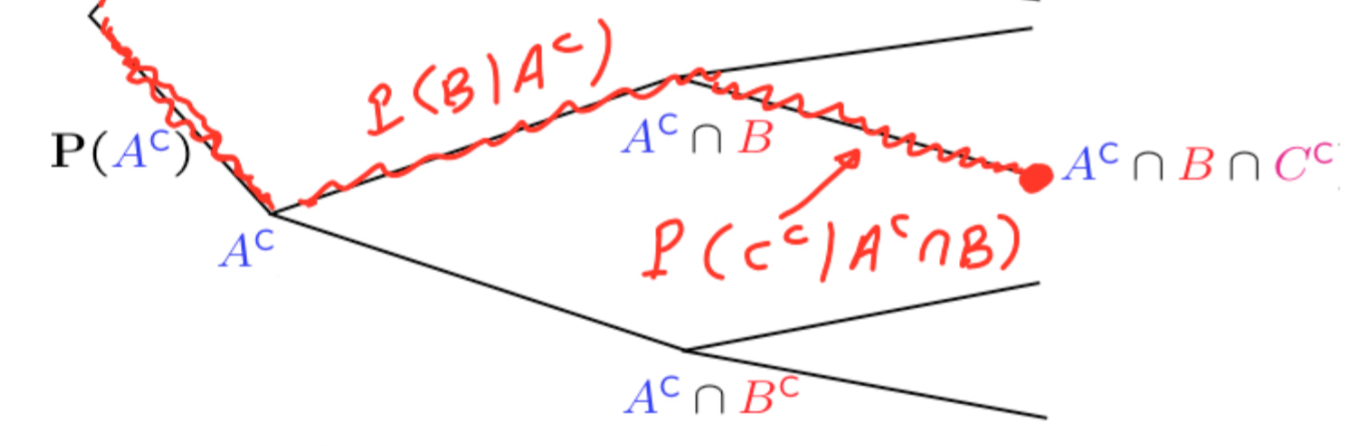
\includegraphics{LowerHalfTree}
  \caption{Lower part of the same tree as in Figure 14. We multiply the probabilities associated with the branches traced in red to get the probability of the event $A^c \cap B \cap C^c$.}
  \setfloatalignment{b}
\end{marginfigure}

\vspace{0.2cm}
At this point, you can probably see that such a formula should also be valid for the case of
more than three events. The probability that a bunch of events all occur should be the probability of the
first event times a number of factors, each corresponding to a branch in a tree of this kind.

In particular, the probability that events $A_1, A_2, \ldots A_n$ all occur is going to be 
\begin{align*}
P(A_1 \cap A_2 \cap \ldots A_n) = P(A_1) \ \prod_{i = 2}^n P (A_i \mid A_1 \cap \ldots \cap A_{i-1})
\end{align*}


This is the most general version of the multiplication rule and allows you to calculate the probability
of several events happening by multiplying probabilities and conditional probabilities.



\newthought{\textit{Check Your Understanding: }} Are the following statements true or false? 
(Assume that all conditioning events have positive probability.)
\begin{enumerate}
\item $P(A \cap B \cap C^c) = P(A \cap B) P(C^c \mid A \cap B)$
\item $P(A \cap B \cap C^c) = P(A) P( C^c \mid A) P( B \mid A \cap C^c)$
\item $P(A \cap B \cap C^c) = P(A) P( C^c \cap A \mid A) P( B \mid A \cap C^c)$
\item $P(A \cap B \mid C) = P( A \mid C) P( B \mid A \cap C)$
\end{enumerate}




\vspace{0.4cm}
\section{The Total Probability Theorem}\label{sec:TotalProb}



Let us now revisit the second calculation that we carried out in the context of our earlier example. In
that example, we calculated the total probability of an event that can occur under different scenarios.
And it involves the powerful idea of divide and conquer where we break up complex situations into
simpler pieces.

\begin{marginfigure}
  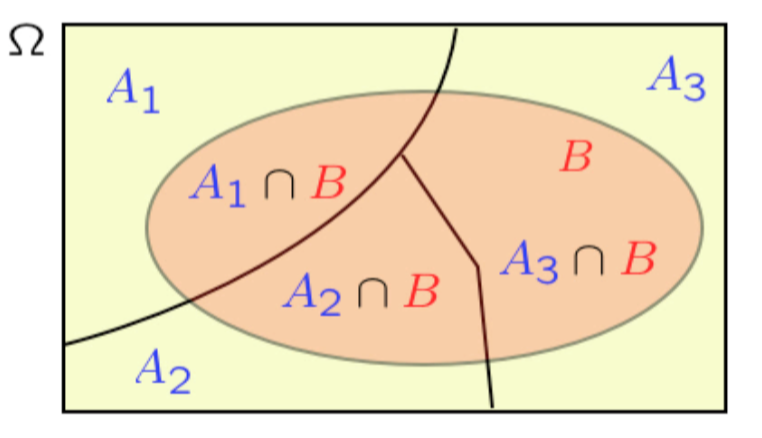
\includegraphics{TotalProb}
  \caption{Decomposing $\Omega$ into non-overlapping events to compute the total probability.}
  \setfloatalignment{b}
\end{marginfigure}


Here is what is involved. We have our sample space which is partitioned into a
number of subsets (we can call these subsets events, as usual). In Figure 16 we take that number to be 3, so we'll have it partitioned into
three possible scenarios. By "partitioned" we mean that 1) these three events cover the entire sample space
and 2) that they're disjoint from each other. Moreover, for each one of the scenarios we're given their probabilities: $P(A_1), P(A_2), P(A_3)$ are known.

If you prefer, you can also draw this situation in terms of a tree. There are three different scenarios that
can happen. We're interested in a particular event, $B$. That event $B$ can happen in three different ways, And these 
three ways correspond
to these particular sub-events $A_1 \cap B, A_2 \cap B \text{ and } A_3 \cap B$ and those are also the labeled leaves in Figure 17.

\begin{marginfigure}
  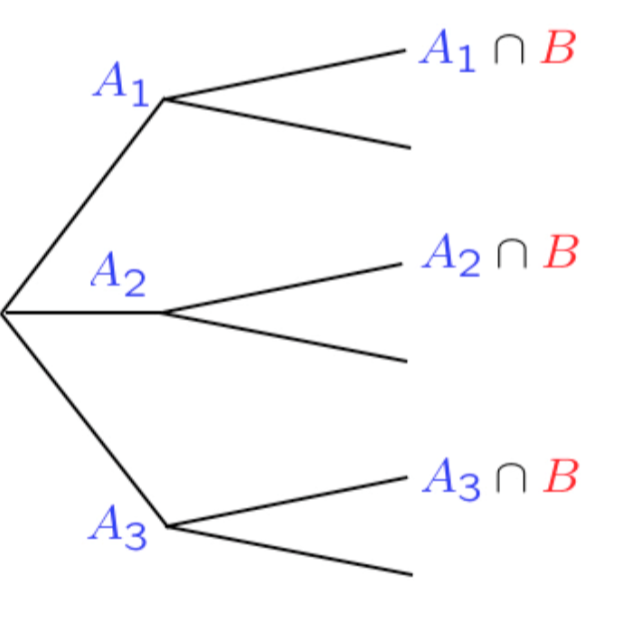
\includegraphics[scale = 0.3]{TotalProbAsTree}
  \caption{Partitioning of $\Omega$ can also be represented as a tree.}
  \setfloatalignment{b}
\end{marginfigure}


\vspace{0.2cm}
Finally, we are given conditional probabilities that event $B$ will materialize under each one of the
different possible scenarios. So we know $P(B \mid A_i)$ for every $i$.


Under those circumstances, can we calculate the probability of event $B$? Of
course we can. And here's how we do it.


First we realize that event $B$ consists of a number of disjoint pieces. One piece is when event $B$ occurs
together with event $A_1$. Another piece is when event $B$ occurs together with $A_2$. Another piece is when
event $B$ occurs together with $A_3$. These three sets are disjoint from each other, as we see in Figure 16. 
And together they form the event $B$. Therefore, the probability of $B$ is going to be, by the
additivity axiom of probabilities, equal to the sum of the probabilities of these sub-events:

$$
P(B) = P(A_1 \cap B) + P(A_2 \cap B) + P(A_3 \cap B)
$$


Furthermore, for each one of these sub-events we can use the multiplication rule and write their
probabilities as follows:

\begin{align*}
P(B) &= P(A_1 \cap B) + P(A_2 \cap B) + P(A_3 \cap B)\\
       &= P(A_1) P(A_1 \mid B) + P(A_2) P(A_2 \mid B) + P(A_3) P(A_3 \mid B)
\end{align*}


So putting everything together, we have arrived at a formula of the following form. The total probability of event $B$
is the sum of the probabilities of the different ways that $B$ may occur, that is, $B$ occurring under the
different scenarios. And those particular probabilities are the product of the probability of the scenario
times the conditional probability of $B$ given that scenario:

\begin{figure}
  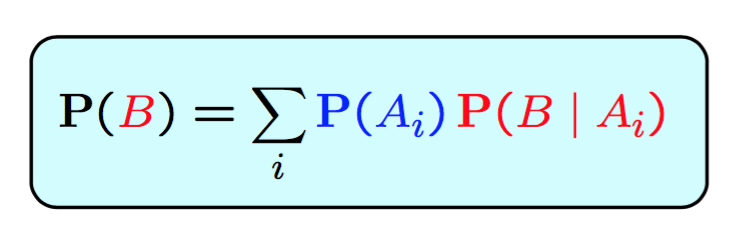
\includegraphics[width=7cm]{TotProbLaw}
  \setfloatalignment{b}
\end{figure}


Now, note that the sum of the probabilities of the different scenarios is of course equal to 1. And this is
because the scenarios form a partition of our sample space. So if we look at this last formula, we
realize that it is a weighted average of the conditional probabilities of event $B$ - weighted average of the
conditional probabilities where the probabilities of the individual scenarios are the weights. In words,
the probability that an event occurs is a weighted average of the probability that it has under each
possible scenario, where the weights are the probabilities of the different scenarios.

One final comment-- our derivation was for the case of three events. But you can certainly see that the
same derivation would go through if we had any finite number of events. But even more, if we had a
partition of our sample space into an infinite sequence of events, the same derivation would still go
through, except that in this place in the derivation, instead of using the ordinary additivity axiom we
would have to use the countable additivity axiom. But other than that, all the steps would be the same.
And we would end up with the same formula, except that now we would have an infinite sum over the
infinite set of scenarios.


\newthought{\textit{Check Your Understanding: }} We have an infinite collection of biased coins, indexed 
by the positive integers. Coin $i$ has probability $2^{-i}$ of being selected. A flip of coin $i$ results in
Heads with probability $3^{-i}$. We select a coin and flip it. What is the probability that the result is Heads? 


The geometric sum formula may be useful here: $\sum_{i = 1}^{\infty} \alpha^i = \frac{\alpha}{1 - \alpha}$, 
when $|\alpha| < 1$.

\vspace{3mm}
\begin{turn}{180} 
\color{teal}
\begin{minipage}{\linewidth}
%Answers:
\scriptsize
theanswerisonefifth
\end{minipage}
\end{turn}




\pagebreak
\section{The Bayes Rule}\label{sec:BayesRule}

We now come to the third and final kind of calculation out of the calculations that we carried out in our
earlier example. The setting is exactly the same as in our discussion of the total probability theorem.
We have a sample space which is partitioned into a number of disjoint subsets, or events, which we think
of as scenarios. We're given the probability of each scenario.

\begin{marginfigure}
  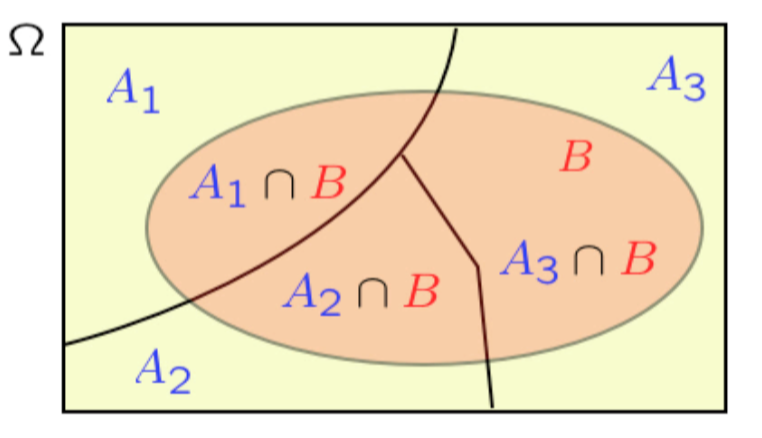
\includegraphics{TotalProb}
  \caption{The setting is exactly the same as in our calculations of total probability.}
  \setfloatalignment{b}
\end{marginfigure}

And we think of these probabilities $A_i$ as being some kind of initial beliefs. They capture how likely we
believe each scenario to be. Now, under each scenario, we also have the probability that an event of
interest, event $B$, will occur. Then the probabilistic experiment is carried out, and we observe
that event $B$ did indeed occur.

Once that happens, maybe this should cause us to revise our beliefs about the likelihood of the different
scenarios. Having observed that $B$ occurred, perhaps certain scenarios are more likely than others.
How do we revise our beliefs? By calculating conditional probabilities.

And how do we calculate conditional probabilities? We start from the definition of conditional
probabilities. The probability of one event given another is the probability that both events occur divided
by the probability of the conditioning event:

\begin{align*}
P(A_i \mid B) = \frac{P(A_i \cap B)}{P(B)}
\end{align*}


How do we continue? We simply realize that the numerator is what we can calculate using the
multiplication rule. And the denominator is exactly what we calculate using the total probability theorem.
So we have everything we need to calculate those revised beliefs, i.e. conditional probabilities.

\begin{figure}
  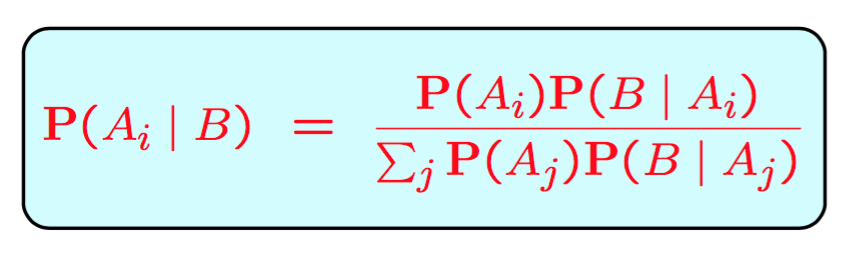
\includegraphics[width=7cm]{BayesRule}
  \setfloatalignment{b}
\end{figure}


And this is all there is in the Bayes rule. It is actually a very simple calculation. However, it is a quite important one.

Its history goes way back. In the middle of the 18th century, a Presbyterian minister, Thomas Bayes,
worked it out. It was published a few years after his death and was quickly reorganized for its
significance. 

Bayes rule is a systematic way for incorporating new evidence, for learning from experience. And it forms the 
foundation of a major branch of mathematics, so-called Bayesian inference, which we will study in some detail 
later in this course. 

The
general idea of Bayesian inference is that we start with a probabilistic model which involves a number of possible scenarios, $A_i$,
and we have some initial beliefs, $P(A_i)$, on the likelihood of each possible scenario. 

There's also some particular event $B$ that may occur under each scenario. And we know how likely it is to
occur under each scenario. 

We then actually observe that $B$ occurred, and then we use that
information to draw conclusions about the possible causes of $B$, or conclusions about the more likely or
less likely scenarios that may have caused this events to occur. That is, having observed $B$, we make inferences as to 
how likely a particular scenario, say $A_i$, is going to be. That likelihood is captured by the conditional probabilities of $A_i$, 
given the event B, that is, by $P(A_i \mid B)$. 


That's exactly what inference is all about, as we're going to see later in this class.


\newthought{\textit{Check Your Understanding: }} A test for a certain rare disease is assumed to be correct 95\% 
of the time: if a person has the disease, the test result is positive with probability 0.95, and if the person does not 
have the disease, the test result is negative with probability 0.95. A person drawn at random from a certain population 
has probability 0.001 of having the disease.

\begin{enumerate}
\item Find the probability that a random person tests positive.
\item Given that the person just tested positive, what is the probability he actually has the disease?
\end{enumerate}
\end{document}


%%%%%%%%%%%%%%%%%%%%%%%%%%%%%%%%%%%%%%%%%%%%%%%%%%%%%%%%%%%%
%%%%%%%%%%%%%%%%%%%%%%%%%%%%%%%%%%%%%%%%%%%%%%%%%%%%%%%%%%%%
%%%%%%%%%%%%%%%%%%%%%%%%%%%%%%%%%%%%%%%%%%%%%%%%%%%%%%%%%%%%

\begin{align}
&P(A) + P(A^c) + P(B) = P(A \cup A^c \cup B) \\
&P(A) + P(B) \leq 1 \\
&P(A^c) + P(B) \leq 1 \\
&P(A \cup B \cup C) \geq P(A \cup B)
\end{align}


\begin{figure}
  
\includegraphics{AxiomConseqHead}
  \setfloatalignment{b}
\end{figure}

%%%%%%%%%%%%%%%%%%%%%%%%%%%%%%%%%%%%%%%%%%%%%%%%%%%%%%%%%%%%

\vspace{0.3cm}


\begin{marginfigure}
  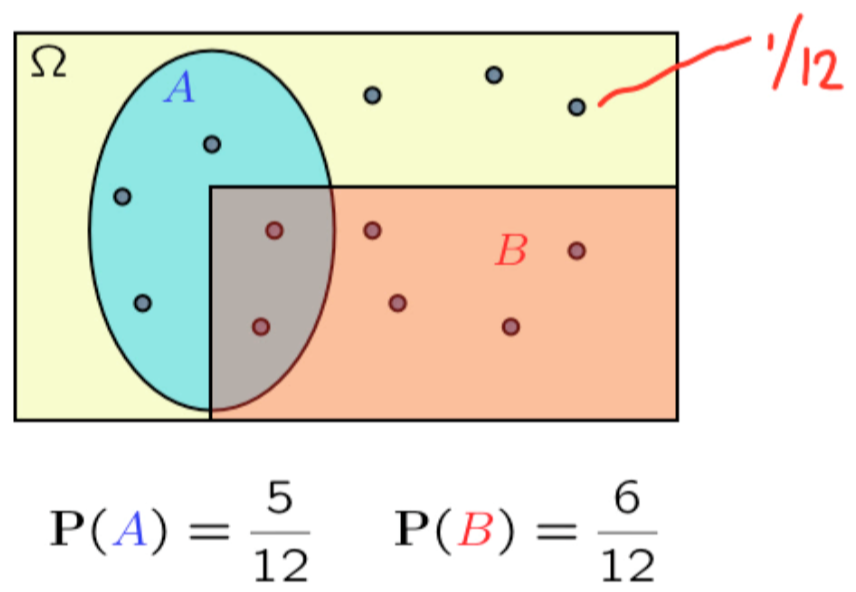
\includegraphics{Cond1}
  \caption{\textbf{Discrete Uniform Law.} Here $\Omega$ has finite number of elements, $n$, and each is equally likely to occur, 
  that is, each has probability of $\frac{1} {n}$ of occurring. Set $A$ contains $k$ elements. Then $P(A) = k \cdot \frac{1} {n} = \frac{k} {n} $ .}
  \setfloatalignment{b}
\end{marginfigure}


%%%%%%%%%%%%%%%%%%%%%%%%%%%%%%%%%%%%%%%%%%%%%%%%%%%%%%%%%%%%

$$
\text{If } A_1, \ldots, A_K\text{ are disjoint } \implies P( A_1 \cup \ldots \cup A_K) = \sum_{i = 1}^K P(A_i)
$$

%%%%%%%%%%%%%%%%%%%%%%%%%%%%%%%%%%%%%%%%%%%%%%%%%%%%%%%%%%%%

\newthought{\textit{Check Your Understanding: }} Let $A$ and $B$ be events, with $P(A)=0.6$ and $P(B)=0.7$. Can these two events be disjoint?

%%%%%%%%%%%%%%%%%%%%%%%%%%%%%%%%%%%%%%%%%%%%%%%%%%%%%%%%%%%%

\setcounter{equation}{0}
\begin{align}
&P(A \cup B \cup C)  = P(A) + P(A^c \cap B) + P (A^c \cap B^c \cap C) \\
&P((A \cap B) \cup (C \cap A^c)) \leq P(A \cup B \cup C) \\
&P(A \cup B \cup C) = P(A \cap C^c) + P(C) + P(B \cap A^c \cap C^c)
\end{align}

%%%%%%%%%%%%%%%%%%%%%%%%%%%%%%%%%%%%%%%%%%%%%%%%%%%%%%%%%%%%

\vspace{0.5cm}
\subsection{Step 2: Describing Our Beliefs about the Outcomes}\label{sec:probability-space}

%%%%%%%%%%%%%%%%%%%%%%%%%%%%%%%%%%%%%%%%%%%%%%%%%%%%%%%%%%%%

\textit{This actually was the proof for the case of three events.} 

